\documentclass{standalone}
\usepackage{pgfplots}
\pgfplotsset{compat=1.17}
\usepackage{amsmath}

\begin{document}

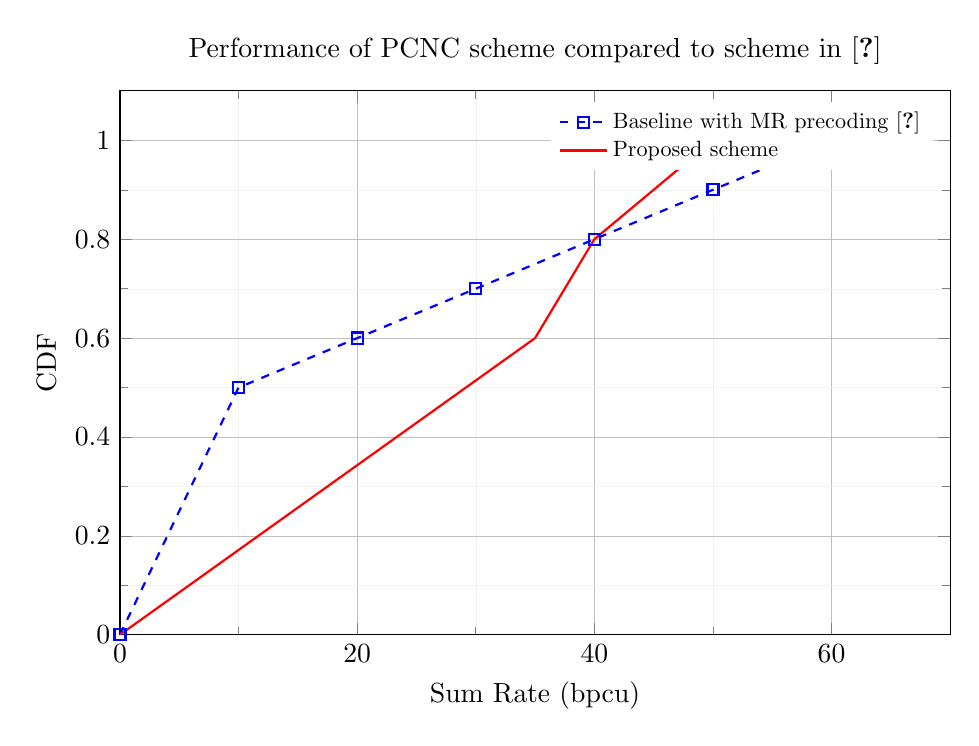
\begin{tikzpicture}
    \begin{axis}[
        title={Performance of PCNC scheme compared to scheme in~\cite{antonioli2023mixed}},
        xlabel={Sum Rate (bpcu)},
        ylabel={CDF},
        xmin=0, xmax=70,
        ymin=0, ymax=1.1,
        xtick={0,20,40,60},
        ytick={0,0.2,0.4,0.6,0.8,1},
        legend pos=north west,
        grid=both,
        grid style={line width=.1pt, draw=gray!10},
        major grid style={line width=.2pt,draw=gray!50},
        minor tick num=1,
        enlargelimits=false,
        width=\textwidth,
        height=0.7\textwidth,
        legend cell align=left,
        legend entries={
            Baseline with MR precoding~\cite{antonioli2023mixed},
            Proposed scheme
        },
        legend style={
            at={(0.98,0.98)},
            anchor=north east,
            nodes={scale=0.8, transform shape},
            draw=none
        }
    ]
        
        % Baseline with MR precoding (dashed blue)
        \addplot[
            color=blue,
            mark=square,
            mark options={solid,fill=blue},
            dashed,
            thick
        ] coordinates {
            (0,0) (10,0.5) (20,0.6) (30,0.7) (40,0.8) (50,0.9) (60,1)
        };
        
        % Proposed scheme (solid red)
        \addplot[
            color=red,
            thick
        ] coordinates {
            (0,0) (35,0.6) (40,0.8) (45,0.9) (50,1) (60,1)
        };
        
    \end{axis}
\end{tikzpicture}

\end{document}